\documentclass[french,a4paper,10pt]{article}

\usepackage[a4paper,hmargin=30mm,vmargin=30mm]{geometry}
\usepackage[T1]{fontenc} % font type
\usepackage[french]{babel} % language
\usepackage{lmodern} % font type
\usepackage[shortlabels]{enumitem}
\usepackage{hyperref}
\usepackage{graphicx}
\usepackage{sectsty}
\usepackage{media9} % for video
%\setlength{\parindent}{0pt}

% compile with pdflatex and evince on linux
% pdflatex compte_rendu.tex -output-directory=out -jobname=compte_rendu && evince out/compte_rendu.pdf
% compile with pdflatex and start on windows
% pdflatex compte_rendu.tex -output-directory=out -jobname=compte_rendu && start out\compte_rendu.pdf



\title{Compte Rendu TPO\\Initiation Blender}
\author{Ivan Lejeune}
\date{\today}


\begin{document}

	\maketitle

	% make table of contents
	\tableofcontents

	\newpage
	\section{Modélisation / Mise en place de la scène}\label{sec:1}

	\subsection{Suppression des éléments de la scène}\label{subsec:1.1}

    On commence par supprimer les éléments de la scène en utilisant la touche \texttt{A} pour tout sélectionner puis
    \texttt{X} pour supprimer.

    \subsection{Ajout d'un sol}\label{subsec:1.2}

    On ajoute un sol en utilisant \texttt{Shift + A} puis \texttt{Mesh (Maillage)} et enfin \texttt{Plane (Plan)}.

    \subsection{Ajout d'un arbre}\label{subsec:1.3}

    On commence par ajouter un cylindre en utilisant \texttt{Shift + A} puis \texttt{Mesh (Maillage)} et enfin
    \texttt{Cylinder (Cylindre)}.

    On modifie les paramètres du cylindre pour obtenir un tronc d'arbre, on a choisit un rayon de 0.1 et une hauteur de
    0.8. On déplace le cylindre pour qu'il soit au dessus du sol (0.8 en hauteur).

    On ajoute ensuite une sphère pour représenter le feuillage de l'arbre, on a choisit un rayon de 0.5. On déplace la
    sphère pour qu'elle soit au dessus du tronc (1.25 en hauteur).

    On duplique l'arbre en sélectionnant les deux éléments (avec \texttt{Shift}) puis en appuyant sur \texttt{Shift + D}
    et \texttt{Enter} pour valider la duplication. On déplace l'arbre dupliqué pour qu'il soit à côté du premier.

    \subsection{Ajout d'une maison}\label{subsec:1.4}

    On commence par ajouter un cube en utilisant \texttt{Shift + A} puis \texttt{Mesh (Maillage)} et enfin
    \texttt{Cube}.

    On modifie les paramètres du cube pour obtenir la base de la maison, on a choisit une longueur de 0.8, une largeur de
    0.55 et une hauteur de 0.4. On déplace le cube pour qu'il soit au dessus du sol (0.4 en hauteur).

    On duplique le cube pour obtenir le toit de la maison, et on le déplace pour qu'il soit au dessus de la base.

    On déforme le toit pour qu'il ait une forme de triangle en allant en mode édition (\texttt{Tab}), en sélectionnant
    \texttt{Glisser les sommets (Shift + V)} puis en déplaçant les sommets du toit.

    On obtient alors la moitié d'un toit, on duplique le toit et on le déplace pour obtenir l'autre moitié.

    \section{Matériaux}\label{sec:2}

    \subsection{Ajout de matériaux}\label{subsec:2.1}

    On ajoute un matériau à tous les éléments de la scène en allant dans l'onglet \texttt{Matériau} puis en cliquant sur
    \texttt{Nouveau}.

    On modifie les paramètres du matériau pour obtenir une couleur verte pour les arbres et une couleur rouge pour la
    maison. On modifie aussi la prévisualisation pour voir les couleurs des matériaux.

    \subsection{Ajout de textures}\label{subsec:2.2}

    On ajoute une texture au sol en allant dans l'onglet \texttt{Texture} puis en cliquant sur \texttt{Nouvelle}.
    On choisit le type de texture \texttt{Image} et on charge une image de texture pour le sol.

    On modifie les paramètres de la texture pour qu'elle soit répétée sur le sol, on modifie aussi la prévisualisation pour
    voir la texture.

    \section{Caméra}\label{sec:3}

    \subsection{Ajout d'une caméra}\label{subsec:3.1}

    On ajoute une caméra en utilisant \texttt{Shift + A} puis \texttt{Camera}.
    On déplace la caméra pour qu'elle soit en face de la scène, on modifie aussi l'angle de vue de la caméra pour qu'elle
    cadre bien la scène.

    \subsection{Ajout d'une contrainte de suivi}\label{subsec:3.2}

    On ajoute une contrainte de suivi à la caméra pour qu'elle suive un objet de la scène.
    On sélectionne la caméra puis l'objet à suivre, on ajoute une contrainte de suivi en allant dans l'onglet
    \texttt{Contraintes} puis en cliquant sur \texttt{Suivi}.

    On modifie les paramètres de la contrainte pour qu'elle suive l'objet en gardant une distance constante.

    \section{Lumière}\label{sec:4}

    \subsection{Ajout d'un soleil}\label{subsec:4.1}

    On ajoute une lumière de type soleil en utilisant \texttt{Shift + A} puis \texttt{Eclairage} et enfin \texttt{Soleil}.
    On déplace la lumière pour qu'elle soit en face de la scène.
    On règle les paramètres de la lumière pour qu'elle donne un effet d'après-midi.
    Pour voir l'effet de la lumière, on peut passer en mode \texttt{Render} en appuyant sur \texttt{F12}.
    On remarque alors que la lumière n'est pas parfaite, on peut essayer un autre type de lumière.

    \subsection{Occlusion ambiante}\label{subsec:4.2}

    On active l'occlusion ambiante en allant dans l'onglet \texttt{Rendu} puis en cochant la case \texttt{Occlusion
    ambiante}.
    On règle les paramètres de l'occlusion ambiante pour qu'elle donne un effet d'après-midi.

    \section{Animation}\label{sec:5}

    \subsection{Ajout d'une "Terre"}\label{subsec:5.1}

    On ajoute une sphère pour représenter la Terre en utilisant \texttt{Shift + A} puis \texttt{Mesh (Maillage)} et enfin
    \texttt{UV Sphere (Sphère UV)}.
    On modifie les paramètres de la sphère pour qu'elle ait une texture de la Terre.

    \subsection{Rebonds de la Terre}\label{subsec:5.2}

    On ajoute une animation pour que la Terre rebondisse en utilisant les \texttt{Keyframes}.
    On sélectionne la Terre puis on se place à la première image de l'animation.
    On ajoute un \texttt{Keyframe} (avec \texttt{i}) pour la position de la Terre.
    On se place à la dernière image de l'animation puis on déplace la Terre vers le haut.
    On ajoute un autre \texttt{Keyframe} pour la position de la Terre.

    On peut alors voir l'animation en passant en mode \texttt{Animation} en appuyant sur \texttt{Alt + A}.

    \section{Rendu}\label{sec:6}

    \subsection{Rendu de la scène en images}\label{subsec:6.1}

    On peut rendre la scène en images en utilisant \texttt{F12}.
    La scène ressemble alors à la figure suivante :
    % insert 2 images of the scene
    \begin{figure}[!htb]
        \begin{minipage}{0.48\textwidth}
            \centering
            \fbox{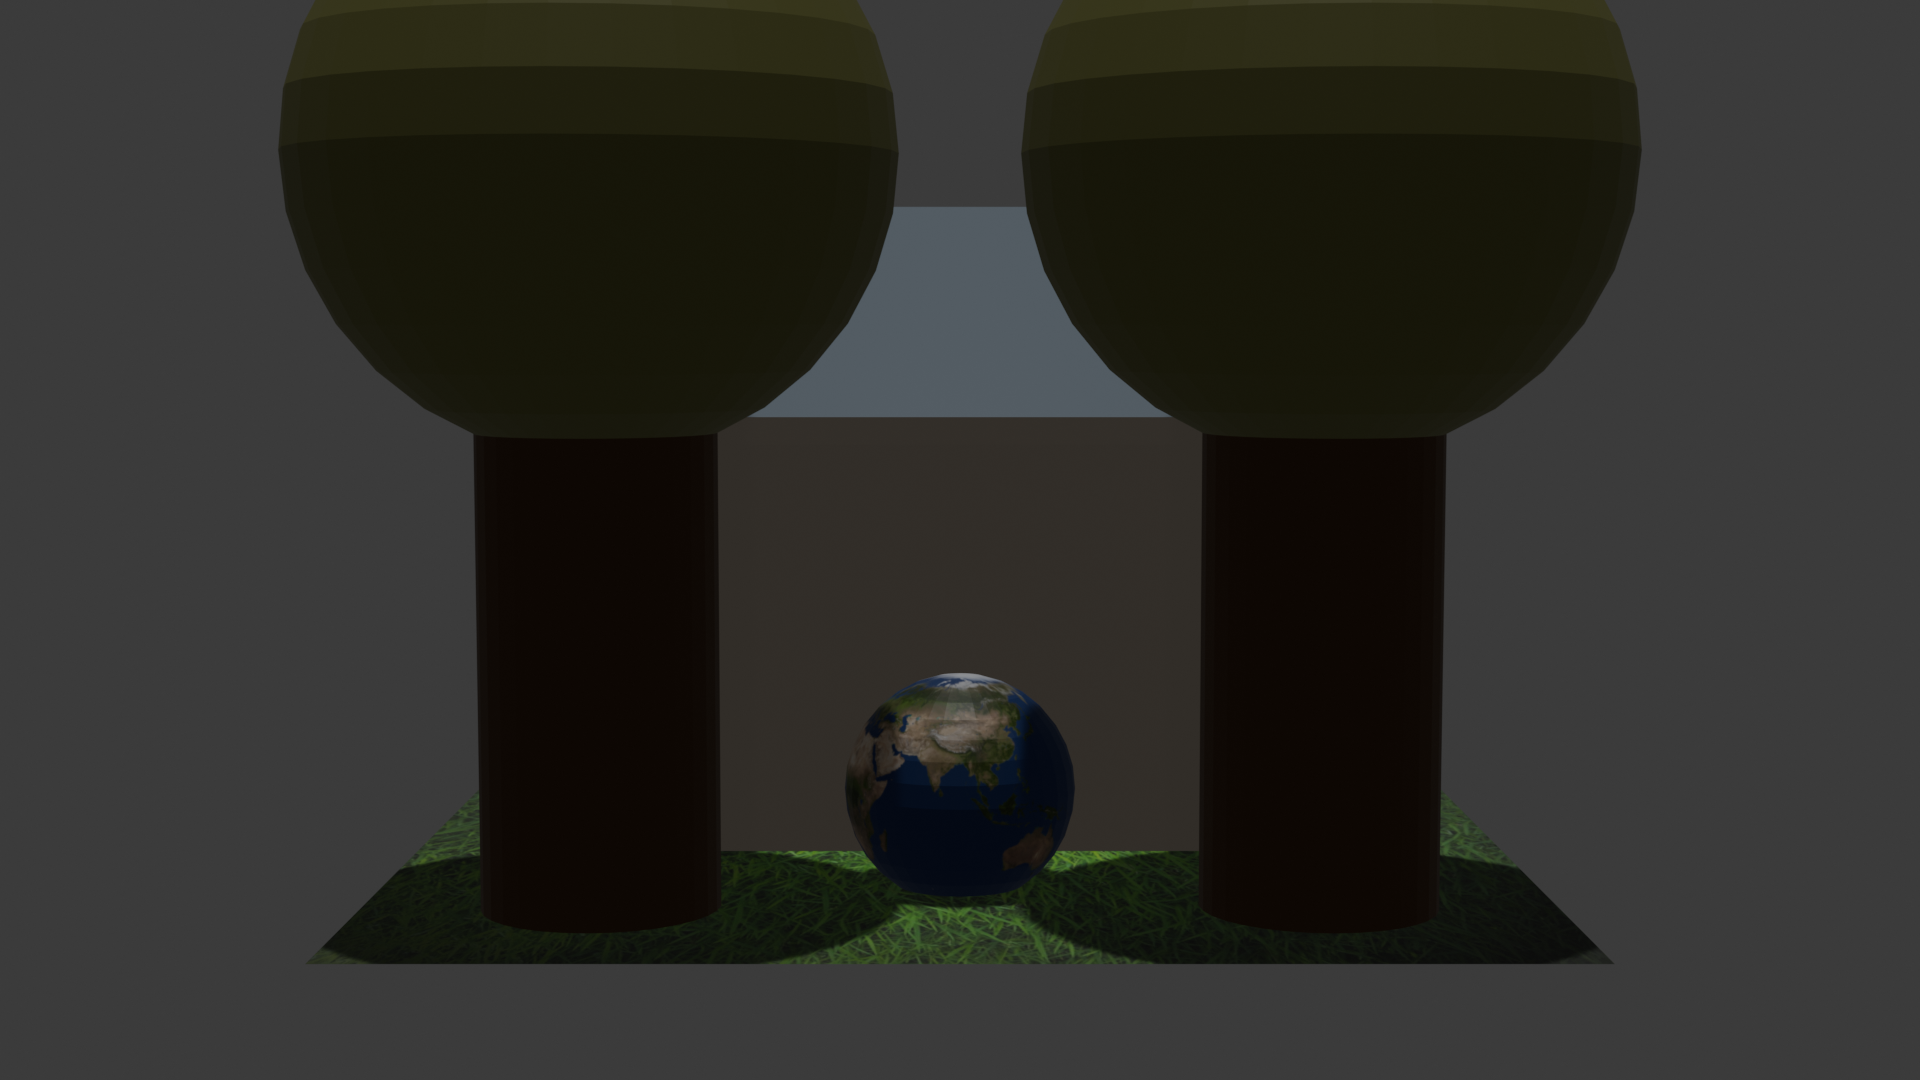
\includegraphics[width=.7\linewidth]{./out/image_rendu}}
            \caption{Vision de la caméra}\label{Fig:scene-1}
        \end{minipage}\hfill
        \begin{minipage}{0.48\textwidth}
            \centering
            \fbox{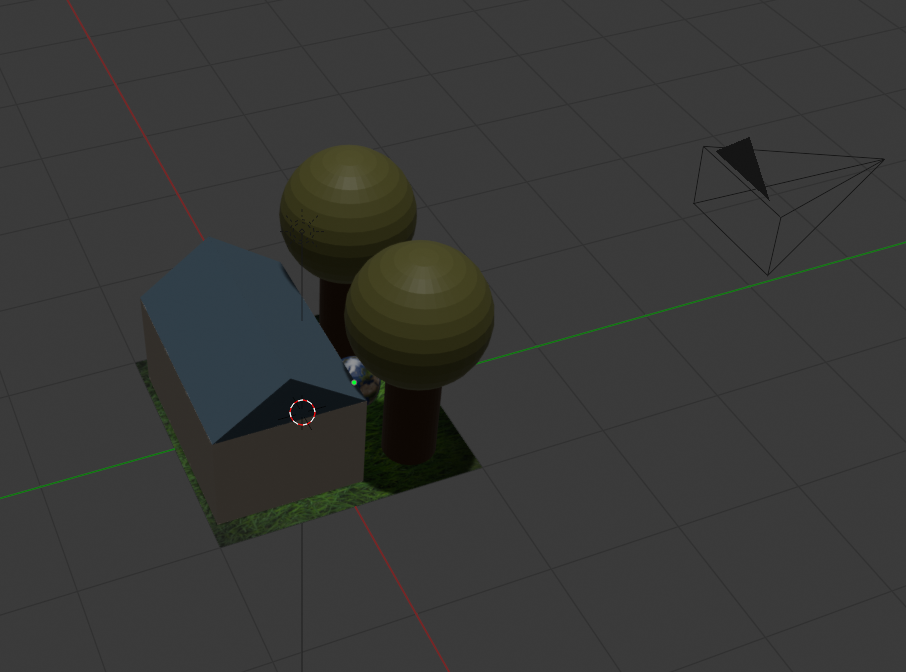
\includegraphics[width=.7\linewidth]{./out/image_rendu_2}}
            \caption{Aperçu global de la scène}\label{Fig:scene-2}
        \end{minipage}
    \end{figure}

    \subsection{Rendu de la scène en vidéo}\label{subsec:6.2}

    On peut rendre la scène en vidéo en utilisant \texttt{Ctrl + F12}.
    On peut alors choisir le format de la vidéo et les paramètres de rendu.
    Sous forme de vidéo, la scène ressemble alors à la figure suivante:
    % insert video of the scene
    pretext
    \includemedia[
	width=0.6\linewidth,
	height=0.4\linewidth,
	activate=onclick,
	addresource=abc.mp4,
	flashvars={
		source=abc.mp4
		&autoPlay=true
		&loop=true
	}
	]{}{VPlayer.swf}
    posttext
    \section{Conclusion}\label{sec:7}

    Ce TP nous a permis de découvrir le logiciel Blender et de nous initier à la modélisation 3D.
    Nous avons pu apprendre à modéliser des objets, à ajouter des matériaux et des textures, à ajouter des caméras et des
    lumières, à ajouter des animations et à rendre des scènes en images et en vidéo.

\end{document}